% Very simple template for lab reports. Most common packages are already included.
\documentclass[a4paper, 11pt]{article}
\usepackage[utf8]{inputenc} % Change according your file encoding
\usepackage{graphicx}
\usepackage{url}
\usepackage{fancyvrb}

%opening
\title{Loggy - a logical time logger}
\author{Chrysoula Dikonimaki}
\date{\today{}}

\begin{document}

\maketitle

\section{Introduction}

This report describes Loggy, a logical time logger implemented in Erlang.

\section{The simple Loggy}
received->sending (when jitter high)
First of all, I ran test:run setting jitter=0. We can see that the order in the ideal case that jitter is 0 is that first will be printed the 'sending' message and then will be printed the 'received' message (see Figure \ref{exp1}).
However, jitter changes this order, as we can see in Figure \ref{exp2}. Decreasing the jitter will reduce the number of messages received in wrong order.

\begin{figure}
  \begin{center}
    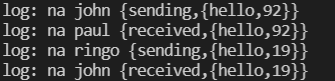
\includegraphics[scale=0.5]{exp1.PNG}
    \caption{Test with jitter=0}
    \label{exp1}
  \end{center}
\end{figure}

\begin{figure}
  \begin{center}
    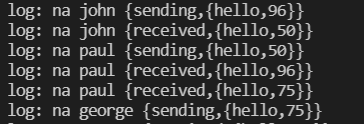
\includegraphics[scale=0.4]{exp2.PNG}
    \caption{Test with jitter=1000}
    \label{exp2}
  \end{center}
\end{figure}

\section{Lamport Time}
\subsection{First Implementation}
In Figure \ref{exp3} we can see a case that the log entries were printed in a wrong order. For example, {hello, 57} has been sent from john to ringo and the received message has been printed before the sent message. It is always true that for each worker the messages has been printed in the right order but we want logger to print all messages in the right order.
\begin{figure}
  \begin{center}
    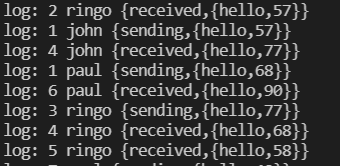
\includegraphics[scale=0.4]{exp3.PNG}
    \caption{Lamport Time, Test with jitter=1000}
    \label{exp3}
  \end{center}
\end{figure}

\subsection{Final Implementation}
\subsubsection{Time Module Description}
Functions:
\begin{itemize}
  \item clock: we will represent our clock as a list of tuples, one tuple per worker node. We will set the time of all tuples (the second entry of each tuple) to 0.
  \item update: replaces the time for a specific worker to the updated time iff the new time is greater than the old one.
  \item safe: we find the min time and check if the message time is less than the min time. If it's true it means that it is safe to log the message.
\end{itemize}
\subsubsection{Test}
At our final implementation all logs are printed in the right order. We can see it in Figure \ref{exp4}. However, we can't be sure that the events have happened in the order shown because some events are concurrent. Concurrent events are events from different processes that it is impossible to know if they have the happened-before relationship.
% TODO: find the max entries in queue

\begin{figure}
  \begin{center}
    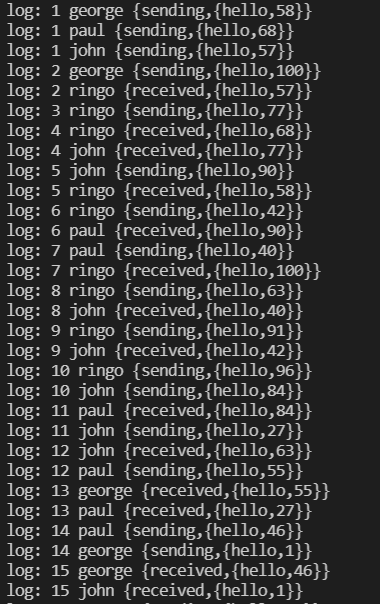
\includegraphics[scale=0.3]{exp4.PNG}
    \caption{Lamport Time Final Implementation, Test with jitter=1000}
    \label{exp4}
  \end{center}
\end{figure}

\subsection{Vector Clocks}
Vector clocks are useful because we can understand if two events are concurrent. The result of testing the vector clock implementation is shown in Figure \ref{exp5}. 

\begin{figure}
  \begin{center}
    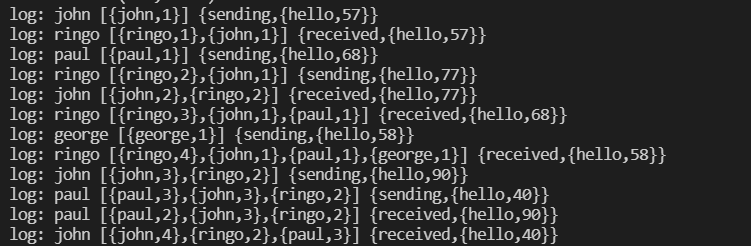
\includegraphics[scale=0.3]{exp5.PNG}
    \caption{Vector Clock Implementation, Test with jitter=1000}
    \label{exp5}
  \end{center}
\end{figure}

\subsection{Maximum number of entries}
I create a new function in the test file called run2 which runs the run function N times and get the average max entries the queue had while running. The results of some tests are shown in Table below.

\begin{center}
\begin{tabular}{ c c c }
Sleep & Jitter & Average max queue size \\
\hline
100 & 1000 & 15.2 \\
100 & 100 & 26.2 \\
100 & 10 & 24.2 \\
1000 & 10 & 13.7  \\ 
\end{tabular}\\
\caption{Results of running the experiment multiple times.}
\label{table_max}
\end{center}

\section{Conclusions}
When it comes to distributed systems, it's difficult to determine the order that the events happen especially, when they don't send messages one another.  
\end{document}
